\documentclass[dvipdfmx]{jsarticle}
\usepackage[dvipdfmx]{graphicx}
\usepackage{amsmath, amssymb}
\usepackage{mathtools}
\usepackage{here}
\renewcommand{\thefigure}{\thesection.\arabic{figure}}
\setcounter{section}{3}
\setcounter{figure}{1}


\begin{document}

\section*{3.1 後半}
(3.4) と (3.5) から,$c(\tau, t)$ は次式で与えられることが必要であることが分かる.

\begin{equation}\label{3.6}
c(\tau, t) = \sum_{n=0}^{N(t)} \alpha_n (t) e^{- \jmath \phi_n (t)} \delta(\tau - \tau_n (t)), \tag{3.6}
\end{equation}

\noindent
ここで,$c(\tau, t)$は時刻$t - \tau$のインパルスに対する時刻$t$のチャネルの等価低域通過応答(ローパスレスポンス)を表す.
\eqref{3.6}を(3.5)に代入すると(3.4)となり,(3.6)がチャネルの等価低域時変インパルス応答であることが確認できる.

\begin{align*}\label{}
r(t) \ &= \ \Re \left\{ \left[ \int_{-\infty}^\infty c(\tau, t) u(t - \tau)d\tau \right] e^{\jmath 2 \pi f_c t} \right\} \\
       &= \ \Re \left\{ \left[ \int_{-\infty}^\infty \sum_{n=0}^{N(t)} \alpha_n (t) e^{- \jmath \phi_n (t)} \delta(\tau - \tau_n (t)) u(t - \tau)d\tau \right] e^{\jmath 2 \pi f_c t} \right\} \\
       &= \ \Re \left\{ \left[ \sum_{n=0}^{N(t)} \alpha_n (t) e^{- \jmath \phi_n (t)} \left( \int_{-\infty}^\infty \delta(\tau - \tau_n (t)) u(t - \tau)d\tau \right) \right] e^{\jmath 2 \pi f_c t} \right\} \\
       &= \ \Re \left\{ \left[ \sum_{n=0}^{N(t)} \alpha_n (t) e^{- \jmath \phi_n (t)} u(t - \tau_n (t))d\tau \right] e^{\jmath 2 \pi f_c t} \right\},
\end{align*}

\noindent
最後の等式はデルタ関数のシフト特性から導かれ,
$\int \delta(\tau - \tau_n (t))u(t - \tau )d\tau = δ(t - \tau_n (t))*u(t) = u(t-\tau_n (t))$ となる.この場合,\eqref{3.6}の和は積分となり,各マルチパス遅延τに関連した時間的に変化する複素振幅に単純化される.

\begin{equation}\label{3.7}
c(\tau, t) = \int \alpha (\xi, t) e^{- \jmath \phi (\xi, t)} \delta(\tau - \xi) d\xi = \alpha(\tau, t)e^{-j\phi(\tau, t)}. \tag{3.7}
\end{equation}

\noindent
時間的に変化するインパルス応答の具体例を挙げると,図3.2のような系で,各マルチパス成分が1つの反射鏡に対応する場合を考えられる.時刻$t_1$において,振幅,位相,遅延の3つ$(\alpha_i, \phi_i, \tau_i), i = 1, 2, 3.$の受信信号に対応する3つのマルチパス成分が存在する.したがって,時間$t_1- \tau_i, i = 1, 2, 3$でチャネルに発射されたインパルスはすべて時間$t_1$で受信され,他の時間にチャネルに発射されたインパルスは$t_1$では受信されない(対応する遅延を有するマルチパス成分が存在しないため).$t_1$に対応する時間変化するインパルス応答は,

\begin{equation}\label{3.8}
c(\tau, t_1) = \sum_{n=0}^{2} \alpha_n e^{- \jmath \phi_n} \delta(\tau - \tau_n) \tag{3.8}
\end{equation}

\noindent
であり,$t = t_1$ のチャネルインパルス応答は図3.3に示すとおりである.図3.2はまた,時刻$t_2$におけるシステムを示しており,振幅,位相,遅延の3つ$(\alpha_i', \phi_i', \tau_i'), i = 1, 2$を有する受信信号に関連する2つのマルチパス成分が存在する.したがって,時間$t_2 - \tau_i',i = 1, 2$にチャネルに発射されたインパルスは,すべて時間$t_2$で受信され,他の時間にチャネルに発射されたインパルスは$t_2$で受信されない.$t_2$における時間変化するインパルス応答は

\begin{equation}\label{3.9}
c(\tau, t_2) = \sum_{n=0}^{1} \alpha_n' e^{- \jmath \phi_n'} \delta(\tau - \tau_n') \tag{3.9}
\end{equation}

\noindent
であり,図3.3にも示されている.

チャネルが時不変であれば,$c(\tau, t)$の時変パラメータは一定となり,$c(\tau, t) = c(\tau)$は単に$\tau$の関数となり,離散的なマルチパス成分を持つチャネルでは,

\begin{equation}\label{3.10}
c(\tau) = \sum_{n=0}^{N} \alpha_n e^{- \jmath \phi_n} \delta(\tau - \tau_n), \tag{3.10}
\end{equation}

\noindent
連続的なマルチパス成分を持つチャネルでは,$c(\tau) = \alpha(\tau)e^{- \jmath \phi(\tau)}$となる.定常チャネルの場合,時間$t_1$のインパルスに対する応答は,時間t2のインパルスに対する応答をシフトしたものになる,$t_1 \neq t_2$.

\begin{figure}[htbp]
\begin{center}
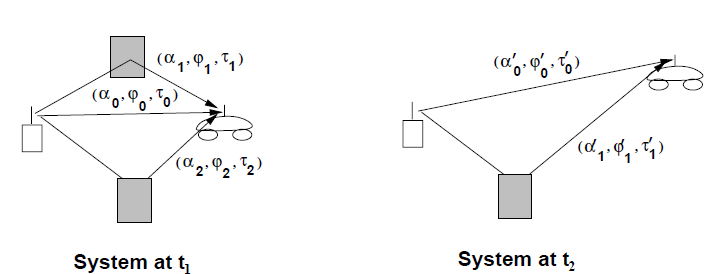
\includegraphics[width=0.8\linewidth]{"./spring_lec/wc_32.png"}
\end{center}
\caption{2つの相違なる測定時間におけるマルチパスの系}
\end{figure}

\begin{figure}[H]
\begin{center}
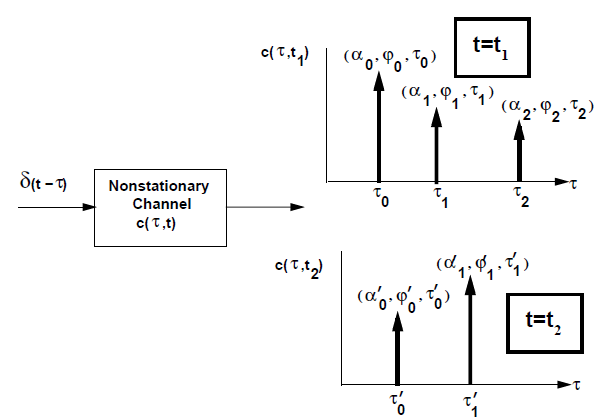
\includegraphics[width=0.7\linewidth]{"./spring_lec/wc_33.png"}
\end{center}
\caption{非定常チャネルの応答}
\end{figure}

一般的な搬送波の周波数では,n番目のマルチパス成分は$f_{c}\tau_n (t) >> 1$となることに注意しなければならない.例えば,$f_c = 1$ GHz,$\tau_n = 50$ ns(屋内系の典型的な値)の場合,$f_{c}\tau_n = 50 >> 1$ となる.屋外の無線システムでは,マルチパスの遅延が50 nsよりもはるかに大きいので,この特性はこれらの系でも成り立つ.$f_{c}\tau_n (t) >> 1$の場合,経路遅延$\tau_n (t)$の小さな変化は,位相$\phi_n (t) = 2\pi f_c \tau_n (t) - \phi_{D_n} - \phi_0 .$のn番目のマルチパス成分において非常に大きな位相変化をもたらす可能性がある.各マルチパス成分の急激な位相変化は,受信信号を構成するマルチパス成分の発展的・破壊的な加算を生じさせ,その結果,受信信号強度が急激に変動する.この現象はフェージングと呼ばれ,以降の章で詳述する.


マルチパスが受信信号に与える影響は,LOSと異なるマルチパス成分に関連する時間の遅延スプレッドが,逆信号帯域幅に対して大きいか小さいかによって決まる.このチャネルの遅延スプレッドが小さい場合,LOSとすべてのマルチパス成分は通常分離できず,次のセクションで説明する狭帯域フェージングモデルにつながる.遅延スプレッドが大きい場合,LOS およびすべてのマルチパス成分は,いくつかの離散成分に分解可能であり,3.3節の広帯域フェージング・モデルにつながる.広帯域モデルにおける離散成分の一部は,分解できない成分で構成されていることに注意が必要である.
遅延スプレッドは,通常,復調装置が同期している受信信号成分に対して測定される.したがって,(3.10)の時不変チャネルモデルにおいて,復調器が最小の遅延$\tau_0$を有するLOS信号成分に同期する場合,遅延スプレッドは定数である$T_m = \max_n \tau_n - \tau_0.$で与えられる.しかし,復調装置が平均遅延$\bar{\tau}$に等しい遅延を有するマルチパス成分に同期する場合,遅延スプレッドは$T_m = \max_n |\tau_n - \bar{\tau}|.$で与えられる.時変チャネルでは,マルチパス遅延は時間と共に変化するので,遅延スプレッド$T_m$はランダム変数となる.さらに,いくつかの受信マルチパス成分は他の成分よりも著しく低い電力を持つので,そのような成分に関連する遅延を遅延スプレッドの特徴付けにどのように使用すべきかは明確ではない.特に,マルチパス成分のパワーがノイズフロア以下であれば,遅延スプレッドに大きく寄与することはないはずである.これらの問題は,3.3.1節で定義されたチャネルパワー遅延プロファイルに対する,遅延スプレッドの特性によって通常対処される.

具体的には,チャネルの遅延スプレッドに関する2つの一般的な特性,平均遅延スプレッドとrms遅延スプレッドは,電力遅延プロファイルから決定される.また,超過遅延スプレッド,遅延ウィンドウ,遅延インターバルのような他の遅延スプレッドの特性評価も使用されることがある[6, Chapter 5.4.1], [28, Chapter 6.7.1].重要なマルチパス成分に関連する遅延をおおまかに測定している限りは,マルチパスチャネルにおける遅延スプレッドの一般的な理解をする上で遅延スプレッドの正確な特性評価はそれほど重要ではない.以下の開発では,遅延スプレッド$T_m$の任意の合理的な特性を使用することが可能だが,一般的にはrms遅延スプレッドを使用することになる.rms遅延スプレッドは,復調装置が平均遅延スプレッドで信号成分に同期すると仮定すると,その平均に関する変動の良い指標となるため,最も一般的な特性評価と言える.チャネル遅延スプレッドは,伝搬環境に大きく依存する.屋内チャネルの遅延スプレッドは通常10~1000ナノ秒,郊外では200~2000ナノ秒,都市部では1~30マイクロ秒の範囲にある[6].

\end{document}